\documentclass{beamer}
\usepackage{amsmath}
\usepackage{amssymb}
\usepackage{bm}
\usepackage{hyperref}
\usepackage{csquotes}

\DeclareSymbolFont{matha}{OML}{txmi}{m}{it}% txfonts
\DeclareMathSymbol{\varv}{\mathord}{matha}{118}
\usetheme{metropolis}

\usefonttheme{serif} % default family is serif

\setbeamertemplate{section in toc}[sections numbered]
\setbeamertemplate{subsection in toc}[subsections numbered]

\title{Macroeconomics 2 Presentation}
\subtitle{Article review :\\ Gabaix, Xavier. 2020. "A Behavioral New Keynesian Model." American Economic Review, 110(8): 2271-2327}
\author{GUGELMO CAVALHEIRO DIAS Paulo \\ MITASH Nayanika \\ WANG Shang}
\institute{Sciences Po}
\date{\today}

\newcommand\ReduceFont{\fontsize{10}{7.2}\selectfont}

\begin{document}

\begin{frame}
    \titlepage
\end{frame}

\begin{frame}
    \ReduceFont
    \frametitle{Outline}
    \tableofcontents[hideallsubsections]
\end{frame}

\section{Introduction}
\begin{frame}
    \tableofcontents[currentsection, hideothersubsections, sections=\value{section}]
\end{frame}

\subsection{Goal of the paper}
\begin{frame}{\subsecname}
    This paper aims to introduce behavioral economics in the New Keynesian model. \\
    \begin{itemize}
        \item \underline{Behavioral Economics} : \\ Since \hyperlink{https://www.jstor.org/stable/1914185}{Kahneman et Tversky (1979)}, aims to introduce deviation to the expected utility theory and the perfect rationality assumption.
        \item \underline{New-Keynesian framework} : \\ General Equilibrium with frictions, what we saw in throughout this class.
    \end{itemize}
    How to integrate coginitive limitations in the New Keynesian model ?
\end{frame}

\subsection{Method of the paper}
\begin{frame}{\subsecname}
\begin{itemize}
    \item Baseline model
    \item Direct conclusions
    \item Consequences on policy
    \item Refinment of the baseline model
    \item Consequences of refinment
\end{itemize}
\end{frame}

\subsection{Conclusions of the paper}
\begin{frame}{\subsecname}
    In a behavioral model :
    \begin{itemize}
        \item Forward guidance is less powerful
        \item The Taylor rule is changed
        \item The equilibrium determinacy is easier to reach
        \item The Zero Lower Bound (ZLB) consequences are changed
        \item The optimal policy are different
        \item Fiscal policies are more powerful
        \item Theoretical contradictions are solved, such as the Neo-Fisherian paradoxes
    \end{itemize}
\end{frame}

\subsection{Literature of the topic}
\begin{frame}{\subsecname}
    Literature on the topic : \\
    \underline{General New Keynesian Framework} : \hyperlink{https://press.princeton.edu/books/hardcover/9780691010496/interest-and-prices}{Woodford 2003b} and \hyperlink{https://perhuaman.files.wordpress.com/2014/06/gali_polc3adtica_monetaria.pdf}{Galí 2015} \\
    \begin{itemize}
        \item \underline{Strength of Forward guidance} : \hyperlink{https://www.newyorkfed.org/medialibrary/media/research/staff_reports/sr574.pdf}{Del Negro, Giannoni, and Patterson (2015)} and \hyperlink{https://www.aeaweb.org/articles?id=10.1257/aer.20150063}{McKay, Nakamura, and Steinsson (2016)}
        \item \underline{Taylor Principle and Equilibrium determinacy} : \hyperlink{https://www.jstor.org/stable/1912186}{Blanchard and Kahn (1980)}
        \item \underline{ZLB and Equilibrium determinacy} : \hyperlink{https://static1.squarespace.com/static/5e6033a4ea02d801f37e15bb/t/5ee1519d8301bb4c205c46d3/1591824801214/320201.email.pdf}{Cochrane (2018)} on the case of Japan
        \item \underline{Policy optimality} : \hyperlink{https://www.jstor.org/stable/2565488}{Clarida, Galí, and Gertler (1999)}, and rationality of firms
        \item \underline{Neo-Fisherian paradoxes} : \hyperlink{https://static1.squarespace.com/static/5e6033a4ea02d801f37e15bb/t/5ee1519d8301bb4c205c46d3/1591824801214/320201.email.pdf}{Cochrane (2018)} on the inconsistency of the New-Keynesian model
    \end{itemize}
\end{frame}

\begin{frame}{\subsecname}
    \underline{Behavioral economics} : How to incorporate cognitive limits in Macroeconomic models ?
    \begin{itemize}
        \item Limited information updating : \hyperlink{https://pages.stern.nyu.edu/~xgabaix/papers/shrouded.pdf}{Gabaix and Laibson (2002)}, \hyperlink{https://academic.oup.com/qje/article-abstract/117/4/1295/1875955?redirectedFrom=fulltext}{Mankiw and Reis (2002)}
        \item Related differential salience : \hyperlink{https://scholar.harvard.edu/files/shleifer/files/bordalo_et_al-2018-the_journal_of_finance.pdf}{Bordalo et al. (2018)}
        \item Noisy signals : \hyperlink{https://www.ecb.europa.eu/pub/pdf/scpwps/ecbwp1331.pdf}{Ma\`ckowiak and Wiederholt (2015)}, \hyperlink{http://www.columbia.edu/~md3405/Working_Paper_20.pdf}{Caplin, Dean, and Leahy (2017)}
        \item Microfoundation : \hyperlink{https://pages.stern.nyu.edu/~xgabaix/papers/sparsebr.pdf}{Gabaix (2014)}
        \item \underline{\hyperlink{https://www.nber.org/papers/w19368}{Woodford (2013)}} for a literature review on the topic.
    \end{itemize}
    There is a large literature on how to model behavioral agents (check pages 5 and 6 of the articles), but the goal of the present article lies elsewhere.\\
    Rewriting Woodford 2003b and Galí 2015 and being complete in the model and in the policy analysis.
\end{frame}


\section{Baseline model of the paper}
\begin{frame}
    \ReduceFont
    \tableofcontents[currentsection, hideallsubsections]
\end{frame}

\begin{frame}
    \tableofcontents[currentsection, hideothersubsections, sections=\value{section}]
\end{frame}

\subsection{Household's Problem}

\subsubsection{Objective function}
\begin{frame}{\subsecname}
    \begin{equation}\tag{3}
        \label{3}
        U = \mathbb{E}\left[\sum_{t=0}^{\infty}\beta^{t}u(c_t,N_t)\right]
    \end{equation}
    With
    \begin{equation*}
    u(c_t,N_t) = \frac{c^{1-\gamma}-1}{1-\gamma}-\frac{N^{1+\phi}}{1+\phi}
    \end{equation*}
    So we have the following objective function of the household: 
    \begin{equation*}
        U = \mathbb{E}\left[\sum_{t=0}^{\infty}\beta^{t}\left(\frac{c^{1-\gamma}-1}{1-\gamma}-\frac{N^{1+\phi}}{1+\phi}\right)\right]
    \end{equation*}
    Subject to 
  \begin{equation}\tag{4}
        k_{t+1}=(1+r_t)(k_t-c_t+y_t)
    \end{equation} 
with $y_t=w_t\cdot N_{t}+y_{t}^{f}$ and $Y_{i t}=N_{i t} e^{\zeta_t}$ where $\zeta_t$ follows an AR(1) process with mean 0

Deterministic steady state $\bar{c}=\bar{N}=\bar{w}=\bar{y}=1$

    
    
\end{frame}

\subsubsection{State Vector}
\begin{frame}{\subsecname}
Law of motion of state vector
\begin{equation}\tag{5}
    \bm{X}_{t+1}=\bm{G}^{\bm{X}}\left(\bm{X}_{t},\bm{\epsilon}_{t+1}\right)
\end{equation}
Decomposing variables as deviations from steady-state
\begin{align*}
    r_{t} &= \bar{r} + \hat{r}_{t} & y_{t} &= \bar{y} + \hat{y}_{t}
\end{align*}
Where the deviations are functions of the State Vector
\begin{align*}
   \hat{r}_{t} &= \hat{r}(\bm{X}_t) & \hat{y}_{t} &= \hat{y}(N_{t},\bm{X}_{t}) := {w}(\bm{X}_{t})N_{t} + y^{f}(\bm{X}_t)- \bar{y}
\end{align*}
Private financial wealth
\begin{equation}\tag{6}
    k_{t+1}=G^{k}(c_{t},N_{t}, k_{t}, \bm{X}_t):= (1+\bar{r}+\hat{r}(\bm{X}_{t}))(k_{t}+\bar{y}+\hat{y}(N_{t},\bm{X}_t)-c_{t})
\end{equation}
\end{frame}

\subsubsection{Linearisation}
\begin{frame}{\subsecname}

Linearisation of the State vector
\begin{equation}\tag{7}
    \bm{X}_{t+1}=\bm{\Gamma}\bm{X}_{t}+\bm{\epsilon}_{t+1}
\end{equation} 
Linearisation of the deviations
\begin{equation*}
    \hat{r}(\bm{X})= \bm{b}_{\bm{X}}^{r} \bm{X}
\end{equation*}

\end{frame}

\subsubsection{Behavioural Model: Discounting of State Variable}
\begin{frame}{\subsecname}
Cognitive Discounting of the State vector (Non-Linearised and Linearised)


\begin{align}
\tag{8}
&\bm{X}_{t+1}=\bar{m}\cdot\bm{G}^{\bm{X}}(\bm{X}_{t},\bm{\epsilon}_{t+1}) \\
\tag{9}
&\bm{X}_{t+1}=\bar{m}(\bm{\Gamma}\bm{X}_{t}+\bm{\epsilon}_{t+1})
\end{align}

Subjective Expectation
\begin{align*}
\mathbb{E}_{t}^{BR}\left[\bm{X}_{t+1}\right]&= \bar{m}\bm{\Gamma}\bm{X_{t}}\\
\mathbb{E}_{t}^{BR}\left[\bm{X}_{t+k}\right]&=\bar{m}^{k}\bm{\Gamma}^{k}\bm{X_{t}}\\
\tag{10}\mathbb{E}_{t}^{BR}\left[\bm{X}_{t+k}\right]&=\bar{m}^{k}\mathbb{E}_{t}\left[\bm{X}_{t+k}\right]
\end{align*}
\end{frame}
\subsubsection{Behavioural Model: Discounting of All Variables}
\begin{frame}{\subsecname}
Cognitive discounting of all Variables (LEMMA 1)
\begin{equation}\tag{11}
    \mathbb{E}_{t}^{BR}\left[z\left(\bm{X}_{t+k}\right)\right]=\bar{m}^{k}\mathbb{E}_{t}\left[z\left(\bm{X}_{t+k}\right)\right]
\end{equation}
For Example
\begin{equation}\tag{12}
    \mathbb{E}_{t}^{BR}\left[\bar{r}+\hat{r}\left(\bm{X}_{t+k}\right)\right]=\bar{r}+\bar{m}^{k}\mathbb{E}_{t}\left[\hat{r}(\bm{X}_{t+k})\right]
\end{equation}

\end{frame}


\subsection{Firm's Problem}

\subsubsection{Firm's Problem}
\begin{frame}{\subsecname}
Firm's Aggregate Price Level

\begin{equation}\tag{13}
    P_{t}=\left(\int_{0}^{1}P_{it}^{1-\varepsilon}\,di\right)^{\frac{1}{1-\varepsilon}}
\end{equation}

Firm's Maximise their real profit
\begin{equation*}
    \nu_{\tau} = \left(\frac{P_{i\tau}}{P_{\tau}}-MC_{\tau}\right)\left(\frac{P_{i\tau}}{P_{\tau}}\right)^{-\varepsilon} c_{\tau}
\end{equation*}
Where
\begin{itemize}
\item    $\left(\frac{P_{i\tau}}{P_{\tau}}\right)^{-\varepsilon} c_{\tau}$ is the total demand for the firm's good 
\item $MC_{t}=(1-\tau_{f})(\omega_{t}/e^{\zeta{t}})=(1-\tau_{f})e^{-\mu_{t}}$ and $\mu_{t} :=\zeta_{t}- \ln \omega_{t}$ is the labour wedge and $\tau_{f}= 1/\varepsilon$ which corrects the price distortions
\end{itemize}
 
    

\end{frame}
\subsubsection{Firm's Real Profits}
\begin{frame}{\subsecname}
Firm's real profit
\begin{equation*}
    \nu_{\tau} = \left(\frac{P_{i\tau}}{P_{\tau}}-MC_{\tau}\right)\left(\frac{P_{i\tau}}{P_{\tau}}\right)^{-\varepsilon} c_{\tau}
\end{equation*}

\begin{equation}\tag{14}
    \nu^{0}(q_{i\tau},\mu_{\tau},c_{\tau}):=\left(e^{q_{i\tau}}-(1-\tau_{f})e^{-\mu_{\tau}}\right)e^{-\varepsilon q_{i\tau}}c_{\tau}
\end{equation} where 
\begin{itemize}
    \item  $q_{i\tau}=\ln\left(\frac{P_{i\tau}}{P_{\tau}}\right)= p_{i\tau}-p_{\tau}$ hence $\left(\frac{P_{i\tau}}{P_{\tau}}\right)= e^{q_{i\tau}}$
\end{itemize}


\end{frame}
\subsubsection{Firm's Real Profits}
\begin{frame}{\subsecname}

$\mathbf{X}_\tau=\left(\mathbf{X}_\tau^{\mathcal{M}}, \Pi_\tau\right)$ where $\Pi_\tau:= p_{\tau}-p_{t}$ and $\mathbf{X}_\tau^{\mathcal{M}}$ is vector including macroeconomic variables.

 If firm hasn't changed its price between $t$ and $\tau$
then its real price $q_{i\tau}= q_{it}- \Pi_{\tau}$ 

Hence the flow of profit 
\begin{equation}\tag{15}
    \nu\left(q_{it},\bm{X}{\tau}\right):=\nu^{0}\left(q_{it}-\Pi(\bm{X}{\tau}),\mu(\bm{X}{\tau}),c(\bm{X}_{\tau})\right)
\end{equation} 

\end{frame}
\subsubsection{Firm's Maximisation Problem}
\begin{frame}{\subsecname}
Maximisation problem for a Traditional Calvo Firm who can adjusts its prices
\begin{equation}\tag{16}
\max_{\text{q}_{it}} \mathbb{E}_{t} \sum_{\tau=t}^{\infty}(\beta\theta)^{\tau-t} \frac{c\left(\bm{X_{\tau}}\right)^{-\gamma}}{\left(\bm{X_{t}}\right)^{-\gamma}} \nu\left(q_{it},\bm{X}{\tau}\right)
\end{equation}
Behavioural Counterpart
\begin{equation}\tag{17}
    \max_{q_{it}}{\mathbb{E}_{t}^{BR} \left[\sum_{\tau=t}^{\infty}(\beta\theta)^{\tau-t}\frac{c\left(\bm{X}_{\tau}^{-\gamma}\right)}{c\left(\bm{X}_{t}^{-\gamma}\right)} \nu\left(q_{it,\bm{X}_{\tau}}\right) \right]}
\end{equation} 
\end{frame}
\subsection{Solution}

\subsubsection{Euler and Static FOC for Labour}
\begin{frame}{\subsecname}
Solving the Household's Maximisation Problem we get:

Euler
\begin{equation}\tag{18}
    \hat{c}_{t}=\mathbb{E}_{t}\left[\hat{c}_{t+1}-\frac{1}{\gamma R}\hat{r}_{t}\right]
\end{equation}

\begin{equation*}
    \hat{c}_{t}=\mathbb{E}_{t}\left[\hat{c}_{t+1}\right]-\sigma\hat{r}_{t}
\end{equation*}

Static First Order Condition for Labour Supply
\begin{equation}\tag{20}
    N^{\phi}_{t}=\omega_{t}c_{t}^{\gamma}
\end{equation}

\end{frame}

\subsubsection{Behavioural Equation}
\begin{frame}{\subsecname}

Using Lemma 1
\begin{equation*}
    \mathbb{E}_{t}^{BR}\left[z\left(\bm{X}_{t+k}\right)\right]=\bar{m}^{k}\mathbb{E}_{t}\left[z\left(\bm{X}_{t+k}\right)\right]
\end{equation*}
We get Behavioural Euler Equation
\begin{equation*}
    \hat{c}(\bm{X_{t}})=\mathbb{E}_{t}^{BR}\left[\hat{c}(\bm{X_{t+1}})\right]-\frac{1}{\gamma R}\hat{r}_{t}
\end{equation*}
\begin{equation}\tag{19}
    \hat{c}_{t}=M\cdot\mathbb{E}_{t}\left[\hat{c}_{t+1}\right]-\sigma\hat{r}_{t}
\end{equation} 
here $M=\bar{m}$
\end{frame}

\subsubsection{Natural Economy/Flexible Price Economy}
\begin{frame}{\subsecname}

Natural Rate Output without pricing frictions
\begin{equation}\tag{21}
    \hat{c}_{t}^{n}=\frac{1+\phi}{\gamma+\phi}\zeta_{t}
\end{equation}
\begin{equation}\tag{22}
    \hat{c}^{n}_{t} = M\cdot\mathbb{E}_{t}\left[\hat{c}^{n}_{t+1}\right]-\sigma\hat{r}^{n}_{t}
\end{equation}
Natural Interest Rate (here natural interest is the same as the pure natural interest rate where there are no budget deficits)
\begin{equation}\tag{23}
    r^{n0}_{t}=\bar{r}+\frac{1+\phi}{\sigma(\gamma+\phi)}\left(M\cdot\mathbb{E}_{t}\left[\zeta_{t+1}\right]-\zeta_{t}\right)
\end{equation}
\end{frame}

\subsubsection{Behavioural Discounted Euler}
\begin{frame}{\subsecname}
Behavioural Discounted Euler Equation
\begin{equation}\tag{24}
    x_{t}=M\cdot\mathbb{E}_{t}\left[x_{t+1}\right]-\sigma(\hat{r}_{t}-\hat{r}^{n}_{t})
\end{equation}
\begin{equation}\tag{25}
    x_{t}=M\cdot\mathbb{E}_{t}\left[x_{t+1}\right]-\sigma(i_{t}-\mathbb{E}_{t}\left[\pi_{t+1}\right]-r^{n}_{t})
\end{equation}
 where
\begin{itemize}
    \item $\hat r_{t}= r_{t}- \bar r = (i_{t}-\mathbb{E}_{t}\left[\pi_{t+1}\right]-\bar{r})$
    \item $\hat r_{t}^{n}= r_{t}^{n}- \bar r$ 
    \item Therefore $\hat{r_{t}}-\hat{r}^{n}_{t}=(i_{t}-\mathbb{E}_{t}\left[\pi_{t+1}\right]-\bar{r})$
\end{itemize}

Iterative Version of the Behavioural Discounted Euler Equation

\begin{equation}\tag{26}
    x_{t}=-\sigma\sum_{k\geq 0}{M\cdot \mathbb{E}_{t}\left[\hat{r}_{t+k}-\hat{r}_{t+k}^{n}\right]}
\end{equation}

\end{frame}

\subsubsection{Optimal Behavioural pricing for the firm}
\begin{frame}{\subsecname}
Optimal price for a behavioural firm resetting its price
\begin{equation}\tag{27}
    p^{*}_{t}=p_{t}+(1-\beta\theta)\sum_{k=0}^{\infty}\left(\beta\theta\bar{m}\right)^{k}\cdot\mathbb{E}_{t}\left[\pi_{t+1}+...+\pi_{t+k}-\mu_{t+k}\right]
\end{equation}

where
\begin{itemize}
    \item $p^{*}_{t}= q_{it}+p_{t}$ 
\end{itemize}

\end{frame}

\subsection{Synthesis Of A Behavioral New Keynesian Model}
\subsubsection{Behavioural New Keynesian Curve}
\begin{frame}{\subsecname}
Behavioural IS Curve
\begin{equation}\tag{29}
    x_{t}=M\cdot\mathbb{E}_{t}\left[x_{t+1}\right]-\sigma(i_{t}-\mathbb{E}_{t}\left[\pi_{t+1}\right]-r^{n}_{t})
\end{equation}

Behavioural Philips Curve
\begin{equation}\tag{30}
    \pi_{t}=\beta\cdot M^{f} \mathbb{E}_t\left[\pi_{t+1}\right]+\kappa\cdot x_{t}
\end{equation}
Where
\begin{equation}\tag{31}
    \begin{cases}
        M=\bar{m} \\
        \sigma=\frac{1}{\gamma R} \\
        M^{f}=\bar{m}\left(\theta+\frac{1-\beta\theta}{1-\beta\theta\bar{m}}(1-\theta)\right)
    \end{cases}
\end{equation}

\end{frame}

\subsection{Calibration}
\subsubsection{Calibration}
\begin{frame}{\subsecname}

\centering

\begin{figure}
  \centering
  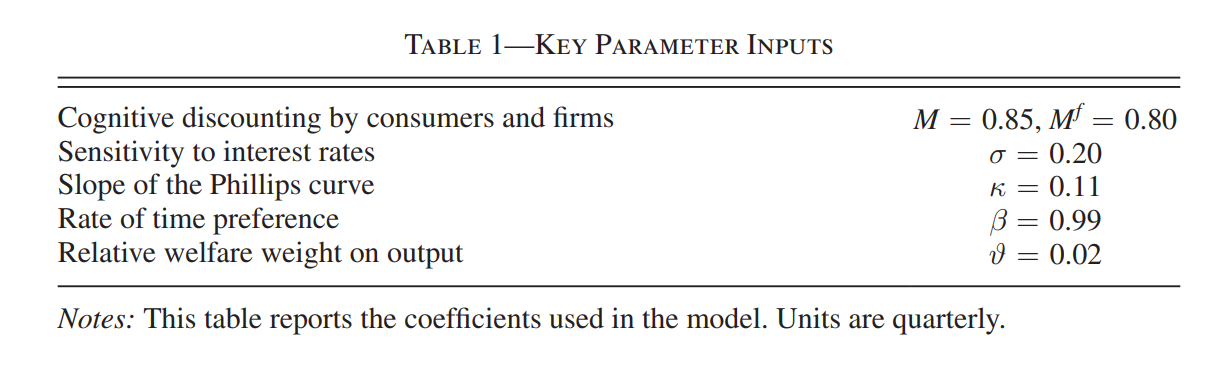
\includegraphics[width=\linewidth]{./Graphs_Macro/Table1.png}
\end{figure}

\begin{figure}
  \centering
  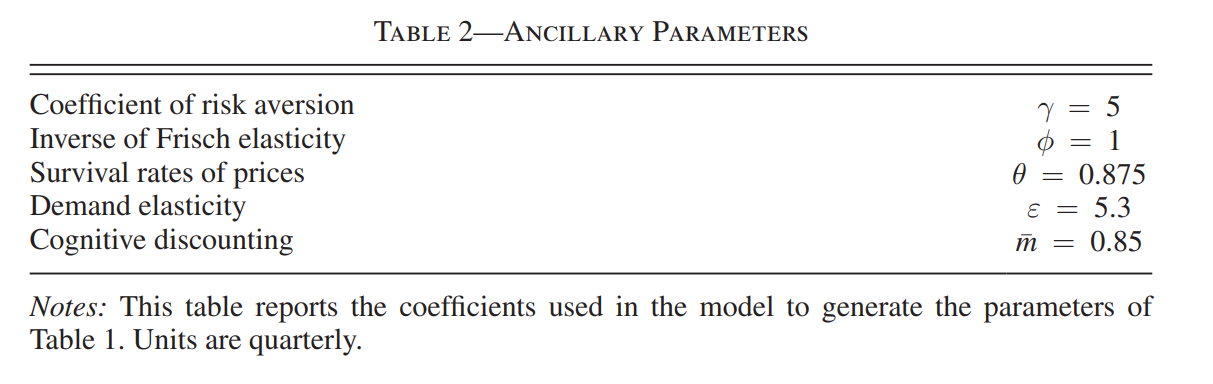
\includegraphics[width=\linewidth]{./Graphs_Macro/Table2.png}
\end{figure}

\end{frame}


\section{Consequences}
\begin{frame}
    \ReduceFont
    \tableofcontents[currentsection, hideallsubsections]
\end{frame}

\begin{frame}
    \tableofcontents[currentsection, hideothersubsections, sections=\value{section}]
\end{frame}

\subsection{The Taylor Principle Reconsidered}

\begin{frame}{\subsecname}
    $\textbf{Rational Model}$: multiple equilibria when monetary policy is passive ($\phi_{\pi}=\phi_{x}=0$).(Note: Taylor Rule: $i_{t}=\phi_{\pi}\pi_{t}+\phi_{x}x_{t}+j_{t}$)\\
    $\textbf{Behavioural Model}$: one unique equilibrium if consumers are myopic enough.\\
    First organize IS and Phillips Curves into matrix form:\\ 
    \begin{equation}\tag{32}                                     \textbf{z}_{t}=\textbf{A}\mathbb{E}_{t}\left[z_{t+1}\right]+\textbf{b}a_{t}
    \end{equation}
    where:
    \begin{itemize}
        \item $\textbf{z}_{t}:=(x_{t},\pi_{t})^{\prime}$
        \item $\textbf{A}=\frac{1}{1+\sigma(\phi_{x}+\kappa\phi_{\pi})}\begin{pmatrix} M & \sigma(1-\beta^{f}\phi_{\pi}) \\ \kappa M & \beta^{f}(1+\sigma\phi_{x})+\kappa\sigma \end{pmatrix}$
        \item $\textbf{b}=\frac{-\sigma}{1+\sigma(\phi_{x}+\kappa\phi_{\pi})}(1,\kappa)^{\prime}$
        \item $a_{t}:=j_{t}-r_{t}^{n}$
    \end{itemize}
\end{frame}

\begin{frame}{\subsecname}
    \textbf{Equilibrium Determinacy with Behavioral Agents} (Propostion 3): There is a determinate equilibrium (i.e., all of $\textbf{A}$’s eigenvalues are less than 1 in modulus) if and only if
    \begin{equation}\tag{34}
        \phi_{\pi}+\frac{(1-\beta M^{f})}{\kappa}\phi_{x}+\frac{(1-\beta M^{f})(1-M)}{\kappa\sigma}>1
    \end{equation}
    When monetary policy is passive, unique equilibrium iff bounded rationality is strong enough:
    \begin{equation}\tag{35}
        \frac{(1-\beta M^{f})(1-M)}{\kappa\sigma}>1
    \end{equation}
\end{frame}

\begin{frame}{\subsecname}
    \textbf{Permanent Interest Rate Peg}. Rational: multiple bounded equilibria. Behavioral: a definite non-explosive equilibrium:
    \begin{equation}\tag{36}
        \textbf{z}_{t}=\mathbb{E}_{t}\left[\sum_{\tau \geq t}\textbf{A}^{\tau-t}\textbf{b}a_{\tau}\right]
    \end{equation}
    \textbf{Long-Lasting Interest Rate Peg}. Rational: very volatile economy. Behavioural: iterating $\textbf{z}_{t}=\mathbb{E}_{t}\textbf{A}_{ZLB}\textbf{z}_{t+1}+\underline{\textbf{b}}$ forward:
    \begin{equation}\tag{37}
        \textbf{z}_{0}(T)=\left(\textbf{I}+\textbf{A}_{ZLB}+...+\textbf{A}_{ZLB}^{T-1}\right)\underline{\textbf{b}}+\textbf{A}_{ZLB}^{T}\mathbb{E}_{0}\left[\textbf{z}_{T}\right]
    \end{equation}
    where:
    \begin{itemize}
        \item $\textbf{A}_{ZLB}$: value of matrix $\textbf{A}$  when $\phi_{\pi}=\phi_{x}=j=0$.
        \item $\underline{\textbf{b}}:=\left(1,\kappa\right)\sigma\underline{r}$
        \item $\underline{r}\leq 0$ is the real interest rate that prevails during the ZLB.
    \end{itemize}
\end{frame}

\subsection{ZLB Is Less Costly with Behavioral Agents}

\begin{frame}{\subsecname}
    \textbf{Rational Model}: Suppose ZLB lasts for T periods and $x_{0}\left(T\right)$ is output gap at time 0. Unboundedly intense recession as $T\to\infty$:
    \begin{equation}\notag
        \lim\limits_{n\to\infty}x_{0}\left(T\right)=-\infty
    \end{equation}
    \textbf{Behavioural Model} (Propostion 4): boundedly intense recession.
    \begin{equation}\tag{38}    \lim\limits_{T\to\infty}x_{0}\left(T\right)=\frac{\sigma\left(1-\beta M^{f}\right)}{\left(1-M\right)\left(1-\beta M^{f}\right)-\kappa\sigma}\underline{r}\textless 0
    \end{equation}
    Myopia has to be stronger when agents are highly sensitive to the interest rate (high $\sigma$ ) and price flexibility is high (high $\kappa$ ). High price flexibility makes the system very reactive, and a high myopia is useful to counterbalance that.
\end{frame}

\begin{frame}{\subsecname}
    \begin{figure}
        \centering
        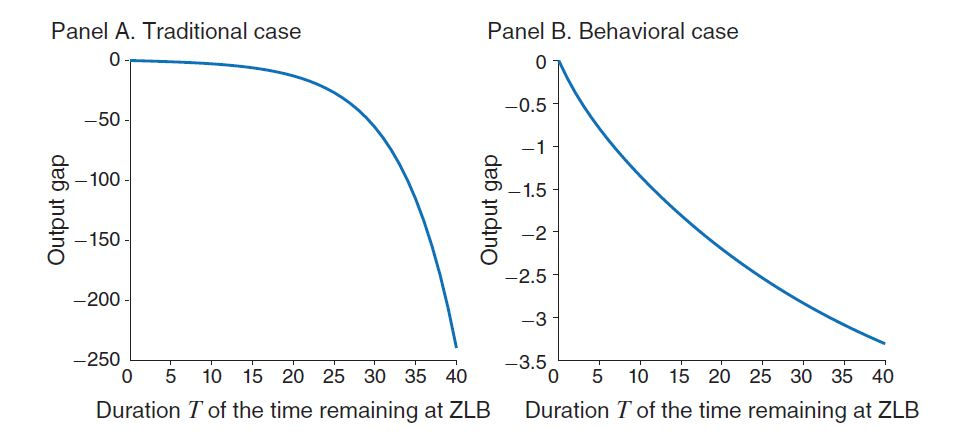
\includegraphics[scale=0.8]{Graphs_Macro/Figure1.JPG}
        \caption{Rational vs Behavioural Models}
        \label{fig:1}
    \end{figure}
    This figure shows the output gap $x_{0}(T)$ at time 0, given that the economy will be at the ZLB for T more periods.
\end{frame}

\subsection{Forward Guidance Is Much Less Powerful}

\begin{frame}{\subsecname}
    \begin{figure}
        \centering
        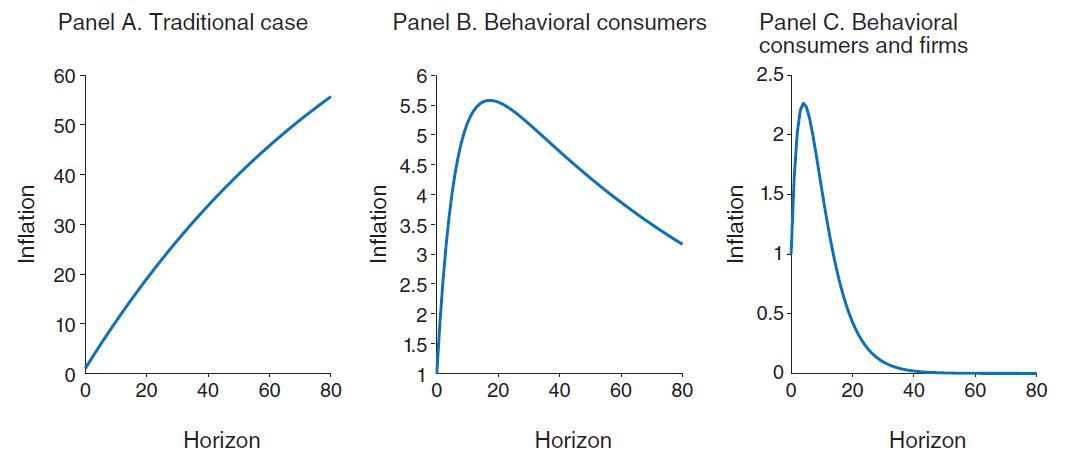
\includegraphics[scale=0.7]{Graphs_Macro/Figure2.JPG}
        \caption{Rational vs Behavioural Models}
        \label{fig:2}
    \end{figure} 
    This figure shows the response of current inflation to forward guidance about a one-period interest rate cut in T quarters, compared to an immediate rate change of the same magnitude.
\end{frame}

\section{Implications for monetary policy}
\begin{frame}
    \ReduceFont
    \tableofcontents[currentsection, hideallsubsections]
\end{frame}

\begin{frame}
    \tableofcontents[currentsection, hideothersubsections, sections=\value{section}]
\end{frame}

\subsection{Welfare with Behavioral Agents and the Central Bank’s Objective}

\begin{frame}{\subsecname}
    Setup: The welfare loss from inflation and output gap is:
    \begin{equation}\tag{39}
        W=-K\mathbb{E}_{0}\sum_{t=0}^{\infty}\frac{1}{2}\beta^{t}\left(\pi_{t}^{2}+\vartheta x_{t}^{2}\right)+W_{-}
    \end{equation}
    where:
    \begin{itemize}
        \item $\widetilde{W}=W^{*}+W$. $W^{*}$ is first best welfare, and W is the deviation from the first best.
        \item $\vartheta=\frac{\overline{\kappa}}{\epsilon}$
        \item $K=u_{c}c\left(\gamma+\phi\right)\left(\epsilon/\overline{\kappa}\right)$
        \item $W_{-}$ is a constant.
        \item $\overline{\kappa}$ is the Phillips curve coefficient with rational firms.
        \item $\epsilon$ is the elasticity of demand.
    \end{itemize}
\end{frame}

\subsection{Optimal Policy with No ZLB Constraints}

\begin{frame}{\subsecname}
    Suppose productivity or discount factor shocks $\Rightarrow$ changes real interest rate: $r_{t}^{n} = r_{t}^{n0}$.\\
    \hfill \linebreak
    \textbf{First-best policy}: zero output gap and inflation \\$\Rightarrow$ $i_{t}=r_{t}^{n0}$ (nominal rate perfectly tracks real rate) \\$\Rightarrow$ true with both rational and behavioral agents (as long as ZLB doesn’t bind $r_{t}^{n0}\geq 0$)\\
    \hfill \linebreak
    Such shocks (\textbf{productivity and discount rate shocks}) allowed monetary
    policy to attain the first best.
\end{frame}

\subsection{Optimal Policy with Complex Trade-Offs}

\begin{frame}{\subsecname}
    Now consider a shock that does \textbf{not} allow the monetary policy to reach the first best: “cost-push shock,” i.e., a disturbance $\nu_{t}$ to the Phillips curve.\\
    \hfill \linebreak
    $\pi_{t}=\beta M^{f} \mathbb{E}t\left[\pi_{t+1}\right]+\kappa x_{t}+\nu_{t}$, with $\nu_{t}$ following a AR(1) process: $\nu_{t}=\rho_{\nu}\nu_{t-1}+\sigma_{t}^{\nu}$ with $\rho_{\nu}\in[0,1)$\\
    \hfill \linebreak
    Examine optimal policies for \textbf{``Commitment''} policy and \textbf{``discretionary''} policy.
\end{frame}

\begin{frame}{\subsecname}
    \textbf{Optimal Policy with Commitment} (Propostion 5).To fight a time-0 cost-push shock, the optimal commitment policy entails, at time $t \geq 0$ :
    \begin{equation}\tag{40}
        \pi_{t}=\frac{-\vartheta}{\kappa}\left(x_{t}-M^{f}x_{t-1}\textbf{1}_{t\textgreater 0}\right)
    \end{equation}
    so that the (log) price level ( $p_{t}=\sum\limits_{\tau=0}^{t}\pi_{\tau}$, normalizing the initial log price level to $p_{-1}$=0) satisfies:
    \begin{equation}\tag{41}
        p_{t}=\frac{-\vartheta}{\kappa}\left(x_{t}+\left(1-M^{f}\right)\sum_{\tau=0}^{t-1}x_{\tau}\right)
    \end{equation}
\end{frame}

\begin{frame}{\subsecname}
    \textbf{Rational Model}. “Price-Level Targeting” is optimal since it ensures that the price level mean-reverts to a fixed target: $p_{t}=(-\nu/\kappa)x_{t}\to0$ in the long run.\\
    \hfill \linebreak    
    \textbf{Behavioural Model}. “Price-Level Targeting” is \textbf{NOT} optimal. Price level is higher after a positive cost-push shock: optimal policy does not seek to bring price level back to baseline.\\    
\end{frame}

\begin{frame}{\subsecname}
    This figure shows the optimal interest rate policy in response to a cost-push shock ($\nu_{t}$), when the central bank follows the optimal commitment strategy.    
    \begin{figure}
        \centering
        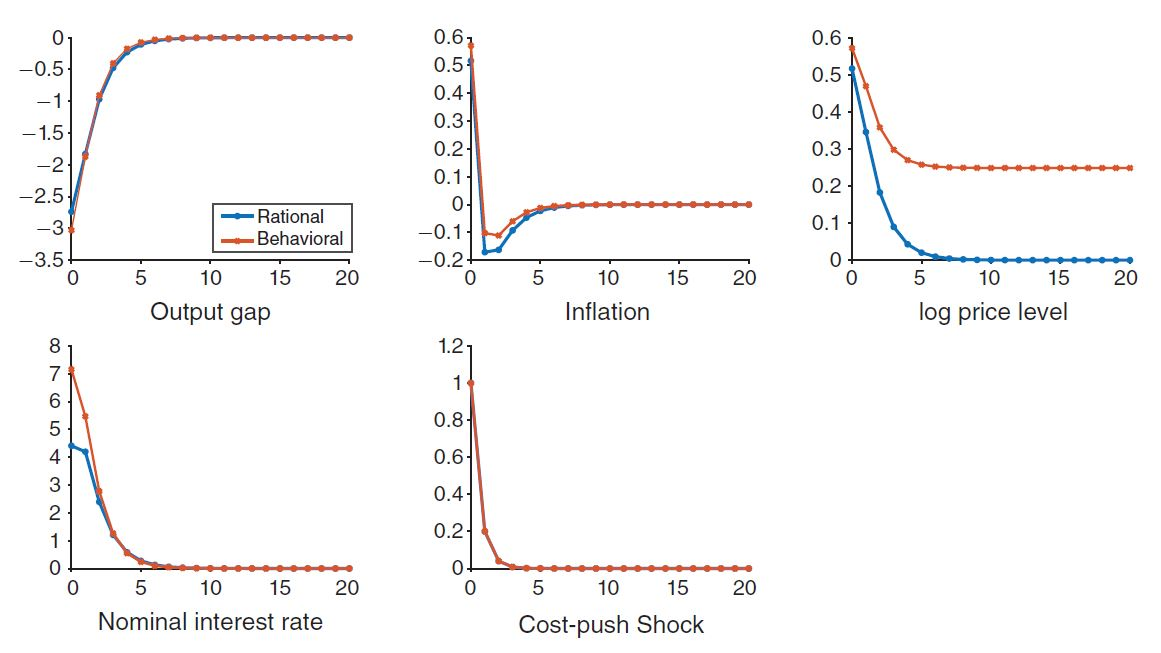
\includegraphics[scale=0.6]{Graphs_Macro/Figure3.JPG}
        \caption{Rational vs Behavioural Models}
        \label{fig:3}
    \end{figure}
\end{frame}

\begin{frame}{\subsecname}
    $\textbf{Optimal Discretionary Policy}$ entails:
    \begin{equation}\tag{42}
        \pi_{t}=\frac{-\vartheta}{\kappa}x_{t}
    \end{equation}
    so that on the equilibrium path: $i_{t}=K\nu_{t}+r_{t}^{n}$, with $K=\frac{\kappa\sigma^{-1}\left(1-M\rho_{\nu}\right)+\vartheta\rho_{\nu}}{\kappa^{2}+\vartheta\left(1-\beta M^{f}\rho_{\nu}\right)}$\\
    \hfill \linebreak
    For persistent shocks ($\rho_{\nu} \textgreater 0$), the optimal policy is less aggressive (K is lower) when firms are more behavioral: future cost-push shocks do not affect much the firms’ pricing today, hence the central bank needs to respond less to them.\\
    \hfill \linebreak      
    Myopia does \textbf{NOT} affect optimal trade-off between inflation and the output gap, but it it does affect the interest rate path that implements this outcome.
\end{frame}

\section{Implications for fiscal policy}
\begin{frame}
    \ReduceFont
    \tableofcontents[currentsection, hideallsubsections]
\end{frame}

\begin{frame}
    \tableofcontents[currentsection, hideothersubsections, sections=\value{section}]
\end{frame}

\subsection{Failure of Ricardian Equivalence}

\begin{frame}{\subsecname}
    The public debt evolves as:
    \begin{equation}\tag{43}
        B_{t+1}=B_{t}+R d_{t}
    \end{equation}
    where:
    \begin{itemize}
        \item $B_{t}$ is the real value of government debt in period t, before period- t taxes.
        \item $d_{t}:=\mathcal{T}_{t}+(r/R)B_{t}$. $d_{t}$ is the budget deficit (after the payment of the interest rate on debt) in period t.
        \item $\mathcal{T}_{t}$ is the lump-sum transfer given by the government to the agent (so that $-\mathcal{T}_{t}$ is a tax).
    \end{itemize}
    No-Ponzi condition is the usual one, $\lim\limits_{t\to\infty}\beta^{t}B_{t}=0$, which here takes the form $\lim\limits_{t\to\infty}\beta^{t}\left(\sum_{s=0}^{t-1}d_{s}\right)=0$. Hence, debt does not necessarily mean-revert, and can follow a random walk.
\end{frame}

\begin{frame}{\subsecname}
    $\textbf{Discounted Euler Equation}$ with Sensitivity to Budget Deficits. Non-Ricardian agents $\Rightarrow$ budget deficits temporarily increase economic activity. The IS curve becomes:
    \begin{equation}\tag{44}            x_{t}=M\mathbb{E}_{t}\left[x_{t+1}\right]+b_{d}d_{t}-\sigma\left(i_{t}-\mathbb{E}_{t}\left[\pi_{t+1}\right]-r_{t}^{n0}\right)
    \end{equation}
    where:
    \begin{itemize}
        \item $r_{t}^{n0}$ is the "pure" natural rate with zero deficits.
        \item $d_{t}$ is the budget deficit.
        \item $b_{d}=\frac{\phi rR(1-\overline{m})}{(\phi+\gamma)(R-\overline{m})}$ is the sensitivity to deficits. When agents are rational, $b_{d}=0$, but with behavioral agents, $b_{d}\textgreater0$.
    \end{itemize}
\end{frame}

\begin{frame}{\subsecname}
    The behavioral IS curve holds, but with the following modified natural rate, which captures the stimulative action of deficits:
    \begin{equation}\tag{45}
        r_{t}^{n}=r_{t}^{n0}+\frac{b_{d}}{\sigma}d_{t}
    \end{equation}
    Hence, bounded rationality gives both a discounted IS curve and an impact of fiscal policy: $b_{d} \textgreater 0$. Deficit-financed (lump-sum) tax cuts have a \textbf{“stimulative” impact on the economy}.
\end{frame}

\subsection{Consequences for Fiscal Policy}

\begin{frame}{\subsecname}
    \textbf{Substitutability of Monetary and Fiscal Policy}. Suppose productivity or discount factor shocks (but no cost-push shocks) that alter the natural rate of interest $r_{t}^{n0}$.First best is achieved if and only if at all dates:
    \begin{equation}\tag{46}
        i_{t}=r_{t}^{n}\equiv r_{t}^{n0}+\frac{b_{d}}{\sigma}d_{t}
    \end{equation}
    where $r_{t}^{n0}$ is “pure” natural rate of interest in (23) and is independent of fiscal and monetary policy.\\
    \hfill \linebreak
    Example: if economy has a lower pure natural interest rate $r_{t}^{n0}$ (hence “needs loosening”), government can: $\downarrow$ interest rates, or $\uparrow$ deficits $\Rightarrow$ Monetary and fiscal policy are perfect substitutes.  
\end{frame}

\begin{frame}{\subsecname}
    \textbf{Fiscal Transfers as an Optimal Cure}, when the ZLB Binds. \\
    \hfill \linebreak
    \textbf{Rational Model}. When the natural rate becomes negative (and with low inflation), the optimal nominal interest rate is negative $\Rightarrow$ first best is not achievable and the second best policy is quite complex.\\
    \hfill \linebreak
    \textbf{Behavioural Model}. Easy first best policy:
    \begin{equation}\tag{47}
        \text{First best at the ZLB: } i_{t}=0 \text{ and deficit: } d_{t}=\frac{-\sigma}{b_{d}}r_{t}^{n0}
    \end{equation}
    i.e., fiscal policy runs deficits to stimulate demand.
\end{frame}

\begin{frame}{\subsecname}
    $\textbf{Government Spending Multiplier Greater than One}$ with Behavioral Agents. Suppose government purchases an amount $G_{t}$ of aggregate good and consumes it. Utility function:
    \begin{equation}\notag
        U(c,N,G) = \frac{c_{t}^{1-\gamma}-1}{1-\gamma} - \frac{N_{t}^{1+\phi}}{1+\phi}+U(G)
    \end{equation}
    Assumes government purchases $G_{0}$ at time 0 financed by a deficit $d_{0}=G_{0}$
    Then the fiscal multiplier is:
    \begin{equation}\tag{48}
        \frac{d Y_{0}}{d G_{0}}=1+b_{d}
    \end{equation}
    reflecting the fact that government spending has a “direct” effect of increasing GDP one-for-one, and then an “indirect” effect of making people feel richer.
\end{frame}


\section{Behavioral Enrichments of the Model}

\begin{frame}
    \ReduceFont
    \tableofcontents[currentsection, hideallsubsections]
\end{frame}

\begin{frame}
    \tableofcontents[currentsection, hideothersubsections, sections=\value{section}]
\end{frame}

\subsection{Term Structure of Consumer Attention}
\begin{frame}{\subsecname}
    It is plausible that consumers \textbf{do not equally pay attention to all economic variables}, even in the present. 
    We could therefore introduce attention discount factors that are variable specific, yielding \textbf{perceived variables} under Bounded Rationality : 
    \begin{itemize}
        \item $\hat{r}^{BR}$ the perceived interest rate under bounded rationality
        \item $\hat{y}^{BR}$ the perceived income under bounded rationality
    \end{itemize}
    Prior to this, consumers perceived perfectly variables at the current period, now, they do not anymore. \\
    \hfill \linebreak
    Directly affects the consumer maximisation program. 
\end{frame}
    
\begin{frame}{\subsecname}
    The law of motion of the personal wealth of the consumer becomes thus a \textbf{perceived law of motion}
    \begin{equation}\tag{6}
        \begin{split}
            k_{t+1}= &\ G^{k}(c_{t},N_{t}, k_{t}, \bm{X}_{t}) \\ 
            & := (1+\bar{r}+\hat{r}(\bm{X}_{t}))(k_{t}+\bar{y}+\hat{y}(N_{t},\bm{X}t)-c_{t})
        \end{split}
    \end{equation}
    Turns into :    
    \begin{equation} \tag{49}
        \begin{split}
            k_{t+1}= &\  \textbf{G}^{k,BR}(c_{t},N_{t},k_{t},\textbf{X}_{t}) \\
            & := (1+\bar{r}+\hat{r}^{BR}(\textbf{X}_t))(k_{t}+\bar{y}+\hat{y}^{BR}(N_{t},\textbf{X}_t)-c_{t})
        \end{split}
    \end{equation}
    \hfill \linebreak
    What could be functional forms of $\hat{r}^{BR}$ and $\hat{y}^{BR}$ ?
\end{frame}

\begin{frame}{\subsecname}
    The perceived values of interest rate and income are defined such that :
    \begin{equation}\tag{50}
        \begin{cases}
            \hat{r}^{BR} = m_{r}\cdot\hat{r}(\textbf{X}_{t}) \\
            \hat{y}^{BR}(N_{t},\textbf{X}_{t}) = m_{y}\cdot\hat{y}(\textbf{X}_{t})+\omega(\textbf{X}_{t})(N_{t}-N_{t}(\textbf{X}_{t}))
        \end{cases}
    \end{equation}
    Equation (50) is a possible functional form. The main changes are the attention discount factor. \\
    Now, what would be the expectation under behavioral expectation of those perceived values ?
\end{frame}

\begin{frame}{\subsecname}
    Consumers already have a general attention discount factor $\bar{m}$, from Lemma 1 in equation (11) :
    \begin{equation*}\tag{11}
        \mathbb{E}_{t}^{BR}\left[z\left(\bm{X}_{t+k}\right)\right]=\bar{m}^{k}\cdot\mathbb{E}_{t}\left[z\left(\bm{X}_{t+k}\right)\right]
    \end{equation*}
    Applied to the perceived interest rate and perceived income, we thus get the \textbf{Lemma 5 (Term Structure of Attention)}:
    \begin{equation}\tag{51}
        \begin{cases}
            \mathbb{E}_{t}^{BR}\left[\hat{r}^{BR}(\textbf{X}_{t+k})\right]=m_{r}\cdot\bar{m}^{k}\cdot\mathbb{E}_{t}\left[\hat{r}(\textbf{X}_{t+k})\right] \\
            \mathbb{E}_{t}^{BR}\left[\hat{y}^{BR}(\textbf{X}_{t+k})\right]=m_{y}\cdot\bar{m}^{k}\cdot\mathbb{E}_{t}\left[\hat{y}(\textbf{X}_{t+k})\right]
        \end{cases}
    \end{equation}
\end{frame}

\begin{frame}{\subsecname}
    What are consequences of this enriched attention structure term ? \\
    When we solve for consumption, we get \textbf{Proposition 8} (Behavioral Consumption Function) :
    \begin{equation}\tag{52}
        \hat{c}_{t}=\mathbb{E}_{t}\left[\sum_{\tau\geq t}\frac{\bar{m}^{\tau-t}}{R^{\tau-t}}\left(b_{r}m_{r}\hat{r}(\textbf{X}_{\tau})+m_{Y}\frac{\bar{r}}{R}\hat{y}(\textbf{X}_{\tau})\right)\right]
    \end{equation}
    With :
    \begin{columns}
        \begin{column}{0.5\textwidth}
            \begin{equation*}
                \begin{cases}
                    c_{t}=c_{t}^{d}+\hat{c}_{t} \\ 
                    c^{d}_{t} = \bar{y} + b_{k}\cdot k_{t} \\
                    b_{k}:=\frac{\bar{r}}{R}\cdot\frac{\phi}{\phi+\gamma} \\ 
                \end{cases}
            \end{equation*}
        \end{column}
        \begin{column}{0.5\textwidth}  %%<--- here
             \begin{equation*}
                \begin{cases}
                    m_{Y}=\frac{\phi\cdot m_{y}+\gamma}{\phi+\gamma} \\
                    b_{r}:=-\frac{1}{\gamma\cdot R^{2}}
                \end{cases}
             \end{equation*}
        \end{column}
    \end{columns}
\end{frame}

\begin{frame}{\subsecname}
    Interest rate has \textbf{direct} and \textbf{indirect} effects on consumption. \\ 
    For a consumer, a decrease in future interest rate : 
    \begin{itemize}
        \item increases their present consumption, because it is more profitable to consume right now (direct effect)
        \item increases other consumers future consumption, increasing their future income, increasing their current consumption (indirect effect)
    \end{itemize}
    Therefore, the aggregate consumption multiplies the positive effect on consumption of a decrease in future interest rate. 
    What does this behavioral model imply for this multiplicator ?
\end{frame}

\begin{frame}{\subsecname}
    In the \textbf{rational consumer} case : \\

    If we derive from equation (52), we get the direct effect : 
    \begin{equation*}
        \Delta^{\text{direct}}:=\frac{\partial \hat{c}_{0}}{\partial \hat{r}_{\tau}}\bigg\rvert_{(y_{t})_{t\geq0 \text{ held constant}}} = -\alpha\cdot \frac{1}{R^{\tau}}
    \end{equation*}
    
    If we derive from equation (26), we get the indirect effect :
    \begin{equation*}
        \Delta^{GE}:=\frac{\partial \hat{c}_{0}}{\partial \hat{r}_{\tau}}=-\alpha R 
    \end{equation*}

    Put together : 
    \begin{equation}\tag{53}
        \frac{\Delta^{GE}}{\Delta^{\text{direct}}}=R^{\tau+1}
    \end{equation}
\end{frame}

\begin{frame}{\subsecname}
    In the \textbf{behavioral consumer} case : \\

    If we derive from equation (52), we get the direct effect : 
    \begin{equation*}
        \Delta^{\text{direct}}:=\frac{\partial \hat{c}_{0}}{\partial \hat{r}_{\tau}}\bigg\rvert_{(y_{t})_{t\geq0 \text{ held constant}}} = -\alpha\cdot m_{r}\cdot\bar{m}^{\tau}\frac{1}{R^{\tau}}
    \end{equation*}

    If we derive from equation (26), we get the indirect effect :
    \begin{equation*}
        \Delta^{GE}:=\frac{\partial \hat{c}_{0}}{\partial \hat{r}_{\tau}}=-\alpha m_{r}\cdot M^{\tau} \frac{R}{R-r\cdot m_{Y}}R 
    \end{equation*}

    Put together : 
    \begin{equation}\tag{54}
        \frac{\Delta^{GE}}{\Delta^{\text{direct}}}=\left(\frac{R}{R-rm_{Y}}\right)^{\tau+1}\in\left[1, R^{\tau+1}\right]
    \end{equation}
\end{frame}

\begin{frame}{\subsecname}
    In a behavioral framework, the multiplicative effect is dampened by bounded rationality. \\

    An attention discount factor that is variable specific allows to explain why forward guidance is not as strong as what theory predicts. \\ 

    What about variable specific attention deficiency for firms now ?
\end{frame}

\subsection{Flattening of the Phillips Curve via Imperfect Firm Attention}
\begin{frame}{\subsecname}
    If we introduce variable specific inattention for firms, equation (15), defining the real profit of the firm : 
    \begin{equation}\tag{15}
        \varv\left(q_{it},\bm{X}{\tau}\right):=\varv^{0}\left(q_{it}-\Pi(\bm{X}{\tau}),\mu(\bm{X}{\tau}),c(\bm{X}_{\tau})\right)
    \end{equation}
    Turns into a perceived real profit of the firm :
    \begin{equation}\tag{55}
        \varv^{BR}(q_{it},(\textbf{X}_{\tau})):=\varv^{0}\left(q_{it}-m^{f}_{\pi}\cdot\Pi(\textbf{X}_{\tau}),m^{f}_{x}\cdot\mu(\textbf{X}_{\tau}),c(\textbf{X}_{\tau})\right)
    \end{equation}
    Where : 
    \begin{itemize}
        \item $m^{f}_{\pi}$ is the attention deficit to inflation 
        \item $m^{f}_{x}$ is the attention deficit to marginal cost
    \end{itemize}
\end{frame}

\begin{frame}{\subsecname}
    The maximisation program of equation (16) :
    \begin{equation}\tag{16}
        \max_{q_{it}} \mathbb{E}_{t}\left[\sum_{\tau=t}^{\infty}(\beta\theta)^{\tau-t} \frac{c\left(\bm{X_{\tau}}\right)^{-\gamma}}{\left(\bm{X_{t}}\right)^{-\gamma}} \varv\left(q_{it},\bm{X}{\tau}\right)\right]
    \end{equation}
    turns into :
    \begin{equation}\tag{56}
        \max_{q_{it}}{\mathbb{E}_{t}^{BR}\left[\sum_{\tau=t}^{\infty}\left(\beta\theta\right)^{\tau-t}\frac{c(\textbf{X}_{\tau})^{-\gamma}}{c(\textbf{X}_{t})^{-\gamma}}\varv^{BR}(q_{it},\textbf{X}_{\tau})\right]}
    \end{equation}
\end{frame}

\begin{frame}{\subsecname}
    Solving it yields :
    \begin{equation}\tag{57}
        \begin{split}
            & p^{*}_{t} = p_{t}+(1-\beta\theta) \cdot \\
            & \sum^{\infty}_{k=0} \left(\beta\theta\bar{m}\right)^{k}\mathbb{E}_{t}\left[m^{f}_{\pi}(\pi_{t+1}+...+\pi_{t+k})-m^{f}_{x}\mu_{t+k}\right]
        \end{split}
    \end{equation}
    In comparison, we had in the baseline model : 
    \begin{equation*}\tag{27}
        p^{*}_{t}=p_{t}+(1-\beta\theta)\sum_{k=0}^{\infty}\left(\beta\theta\bar{m}\right)^{k}\cdot\mathbb{E}_{t}\left[\pi_{t+1}+...+\pi_{t+k}-\mu_{t+k}\right]
    \end{equation*}
\end{frame}

\begin{frame}{\subsecname}
    We also get : 
    \begin{equation*}
        M^{f}=\bar{m}\left(\theta+m^{f}_{\pi}\cdot(1-\theta)\cdot\frac{1-\beta\cdot\theta}{1-\beta\cdot\theta\cdot\bar{m}}\right)\in\left[0,1\right]
    \end{equation*}
    \begin{equation}\tag{58}
        \kappa = m^{f}_{x}\bar{\kappa}
    \end{equation}

    Where 
    \begin{itemize}
        \item $M^{f}$ is the general attention factor of the firm
        \item $m^{f}_{x}$ is the attention deficiency to the output gap
        \item $\kappa=m_{x}^{f}\cdot\bar{\kappa}$, is the perceived value of the importance of outputgap on inflation
    \end{itemize}
\end{frame}

\begin{frame}{\subsecname}
    If we solve the Phillips curve, the equation (29) : 
    \begin{equation}\tag{29}
        \pi_{t}=\beta\cdot M^{f}\cdot\mathbb{E}_{t}\left[\pi_{t+1}\right]+\kappa\cdot x_{t}
    \end{equation}
    Turns into a Phillips Curve with Behavioral Firms, allowing for imperfect attention to inflation and costs (\textbf{Proposition 10}) :
    \begin{equation*}
        \pi_{t}=\beta\cdot\bar{m}\left(\theta+m^{f}_{\pi}\cdot(1-\theta)\cdot\frac{1-\beta\cdot\theta}{1-\beta\cdot\theta\cdot\bar{m}}\right)\cdot\mathbb{E}_{t}\left[\pi_{t+1}\right]+m_{x}^{f}\cdot\bar{\kappa}\cdot x_{t}
    \end{equation*}
\end{frame}

\subsection{Nonconstant Trend Inflation and Neo-Fisherian Paradoxes}
\begin{frame}{\subsecname}
    Now, let's change the way we consider inflation. Instead of a steady state, agents perceive a default value.
    The article proposes the following functional form :
    \begin{equation}\tag{59}
        \pi^{d}_{t}=(1-\zeta)\bar{\pi}_{t}+\zeta\bar{\pi}_{t}^{CB}
    \end{equation}
    The IS curve is unchanged, and is the same as equation (28) :
    \begin{equation}\tag{60}
        x_{t}=M\mathbb{E}_{t}\left[x_{t+1}\right]-\sigma\left(i_{t}-\mathbb{E}_{t}\left[\pi_{t+1}\right]-r^{n}_{t}\right)
    \end{equation}
\end{frame}

\begin{frame}{\subsecname}
    The Phillips curve of equation (29) :
    \begin{equation}\tag{29}
        \pi_{t}=\beta\cdot M^{f} \mathbb{E}_{t}\left[\pi_{t+1}\right]+\kappa\cdot x_{t}
    \end{equation}
    Turns into :
    \begin{equation}\tag{61}
        \hat{\pi}_{t}=\beta\cdot M^{f}\cdot\mathbb{E}_t\left[\hat{\pi}_{t+1}\right]+\kappa\cdot x_{t}
    \end{equation}
    The only difference is through $\hat{\pi}_{t}$, with ${\pi}_{t}=\pi^{d}_{t}+\hat{\pi}_{t}$.
\end{frame}

\begin{frame}{\subsecname}
    Finally, the equilbrium condition changes through $\zeta$ the weight given to the Central Bank declaration. 
    Equation (34) in the Baseline model :
    \begin{equation}\tag{34}
        \phi_{\pi}+\frac{(1-\beta M^{f})}{\kappa}\phi_{x}+\frac{(1-\beta M^{f})(1-M)}{\kappa\sigma}>1
    \end{equation}
    Turns into :
    \begin{equation}\tag{62}
        \phi_{\pi}+\zeta \frac{(1-\beta M^{f})}{\kappa}\phi_{x}+\zeta\frac{(1-\beta M^{f})(1-M)}{\kappa \sigma}>1
    \end{equation}
    The term $\zeta$ can be considered as the weight of central bank guidance.
    \begin{itemize}
        \item What if it is 0 ?
        \item What are the consequences for Central Bankers ?
    \end{itemize}
\end{frame}

\begin{frame}{\subsecname}
    \textbf{\underline{Neo-fisherian neutrality}} : In the long-run, inflation (money) should not affect output. \\
    In the New-Keynesian framework, it does not work : if inflation is permanently higher, then output is permanent higher.
    Let $M^{f}=1$, then :
    \begin{equation}\tag{29}
        \pi_{t}=\beta\cdot M^{f}\cdot\mathbb{E}_{t}\left[\pi_{t+1}\right]+\kappa\cdot x_{t}
    \end{equation}
    Turns in the steady state into :
    \begin{equation*}
        \pi=\beta\cdot\pi+\kappa\cdot x
    \end{equation*}
    $$\iff$$
    \begin{equation*}
        \pi\cdot\frac{1-\beta}{\kappa}= x
    \end{equation*}
\end{frame}

\begin{frame}{\subsecname}
    In the current extension, it is not the case : \\
    Trend in inflation :
    \begin{equation*}
        {\pi}_{t}=\pi^{d}_{t}+\hat{\pi}_{t}
    \end{equation*}
    Perception of the trend :
    \begin{equation}\tag{59}
        \pi^{d}_{t}=(1-\zeta)\cdot\bar{\pi}_{t}+\zeta\cdot\bar{\pi}_{t}^{CB}
    \end{equation}
    Phillips curve :
    \begin{equation}\tag{61}
        \hat{\pi}_{t}=\beta\cdot M^{f}\cdot\mathbb{E}_t\left[\hat{\pi}_{t+1}\right]+\kappa\cdot x_{t}
    \end{equation}
    IS curve :
    \begin{equation}\tag{60}
        x_{t}=M\cdot\mathbb{E}_{t}\left[x_{t+1}\right]-\sigma\left(i_{t}-\mathbb{E}_{t}\left[\pi_{t+1}\right]-r^{n}_{t}\right)
    \end{equation}
    We find $\implies i=r^{n}+\bar{\pi}$ and no impact of long run inflation over output.
\end{frame}

\begin{frame}
    Conclusion of those enrichments :
    \begin{itemize}
        \item Variable specific attention deficiency allows for more detail in the specification.
        \item Allows to highlight even more the conclusions of the general model
        \item Answer both empirical problems and pure theoretical questions
    \end{itemize}
\end{frame}


\section{Discussion of the Behavioral Assumptions, Conclusion, Critics}
\begin{frame}
    \ReduceFont
    \tableofcontents[currentsection, hideallsubsections]
\end{frame}

\begin{frame}
    \tableofcontents[currentsection, hideothersubsections, sections=\value{section}]
\end{frame}

\subsection{Behavioural enrichments}

\begin{frame}{\subsecname}
\textbf{Theoretical Microfoundations:} evidence exists for the inattention to small parameters, but no direct evidence on cognitive discounting. More empirical research on this is required despite the presence of extant evidence. Literature exists on cognitive discounting closely resembling hyperbolic discounting

\textbf{Lucas Critique:} Attention is endogenised in the appendix to reflect the fact that the attention becomes more intense when the volatility/deviation in the environment is more. Lucas critique hence becomes relevant for large changes. 

\end{frame}

\begin{frame}{\subsecname}
\textbf{Long Run Learning:} Learning and Attention is costly and require effort. Hence the agent might not learn anything in the long run. 

\textbf{Parsimony and new variants:} The current model is quite parsimonious and with just one standard parameter; $\bar{m}$. The term structure of attention enriches the model and the measurement of such an attention parameters is better. There is scope for improving the measurement of macro parameter of attention. Reasonable variations are possible for this model and the author chooses an \textit{"a happy balance between tractability, parsimony, and psychological and macroeconomic realism"}
\end{frame}

\subsection{Conclusion}
\begin{frame}{\subsecname}

1. This parsimonious model can be expanded examples include capital accumulation, a more frictional labor market, distortionary taxes, and agents that are heterogeneous in wealth or rationality.

2. Requirement for more empirical work to estimate attention to current variables and future variables.

3. Introduce survey designs which measures people's subjective view of the world. 

\end{frame}

\subsection{Critics}
\begin{frame}{\subsecname}

Overall the paper acknowledges that the model presented is parsimonious and more variations to it can be added. It more or less exhaustively covers the variations while discussing the possible behavioural enrichments. 

However, a few critiques \\
1. While modeling welfare for behavioral agents, the paper does not use subjective expectation. \\
2. It is possible that agents possess heterogeneous beliefs and can have different ways of expressing their partial myopia. \\
3. There is a need for more empirical testing for behavioral parameters, which the paper also acknowledges.


\end{frame}



\end{document}

